% ICASSP 2027 submission. Open items are \tbd{red} so none can reach the PDF unseen.
\documentclass{article}
\usepackage{spconf,amsmath,amssymb,graphicx}
\usepackage{booktabs}
\usepackage{multirow,rotating}
\usepackage{xcolor}
\usepackage[hidelinks]{hyperref}
\usepackage{microtype}

% five floats at the template's default 20pt separation cost most of a column
\setlength{\textfloatsep}{11pt plus 2pt minus 2pt}
\setlength{\floatsep}{11pt plus 2pt minus 2pt}
\setlength{\intextsep}{11pt plus 2pt minus 2pt}
\setlength{\dbltextfloatsep}{11pt plus 2pt minus 2pt}

\newcommand{\tbd}[1]{\textcolor{red}{#1}}
\newcommand{\sys}{CANDOR}

\title{REAL-TIME SCORE FOLLOWING IN SHEET MUSIC IMAGES\\AS SEQUENTIAL CANDIDATE SELECTION}
\name{Pouya Mohseni, Ichiro Fujinaga}
\address{Schulich School of Music, McGill University, Montr\'eal, Canada}

\begin{document}
\maketitle

\begin{abstract}
Score following aligns a live performance to its score in real time, committing
to a position at every instant with no lookahead. The two sides are different
kinds of object, the performance audio and the score an image. The
established response is to convert one into the other and align within a single
modality, either by turning the page into symbols with optical music
recognition or by turning the audio into notes with transcription, and each
detour inherits the errors of its conversion. Sheet-image score following
converts neither side and learns the correspondence directly, and its strongest
systems condition a visual detector on the audio. What limits them is
annotation, since performances aligned to notehead coordinates are costly
enough that nearly all training data is synthesized, so these systems work on
synthesized audio and lose much of their accuracy on a real instrument in a
real room. Closing that gap is the field's central open problem, and every
remedy proposed for it has treated the gap as a failure of perception. We show
it is not. On real recordings the detector already proposes a correct position
at every scored onset, and an oracle held to the same real-time commitments
recovers almost everything the deployed rule loses. We therefore recast the
task as sequential selection over the candidates the detector already emits,
combining a parameter-free transition model with a set-based scorer that judges
each candidate against its competitors in the same instant. This sets a new
best on real piano recordings, holds across three independently trained
detectors, and shows that what the decision needs is its own temporal history
rather than a better image representation.
\end{abstract}

\begin{keywords}
Score following, sheet music, audio-to-score alignment, real-time,
music information retrieval
\end{keywords}

\section{Introduction}
\label{sec:intro}

A musician plays from a printed page; a machine listens, looks at the same
page, and at every moment reports where in the music the performer has got to.
That is score following~\cite{orio2003}, and it is what automatic page
turning~\cite{arzt2008}, live computer
accompaniment~\cite{dannenberg1984,dannenberg2006,raphael2010} and
score-synchronised visualisation are built on.

Aligning a performance to its score offline is a different problem, usually
called audio-to-score alignment or music synchronisation. There the whole
recording is in hand, a global method such as dynamic time warping settles
every position at once~\cite{dixon2005match}, and even repeats and jumps can be
resolved after the fact~\cite{shan2020,morsi2022}. Offline alignment underpins
cross-modal retrieval and piece identification, where a recording is matched
against a collection of scores~\cite{dorfer2018msmd}. Score following, also
called music tracking~\cite{arzt2010}, gets none of that. It sees only what has
been played, commits to a position immediately, and never revises it.
Everything below respects this constraint, including the oracles we use to
measure what is achievable.

The remaining difficulty is that the two sides are different kinds of object.
The performance is audio, the score is an image, and there is no shared space
in which to compare them. The literature answers this in three ways.

\subsection{Related work}
\label{ssec:related}

One family converts the score. Optical music recognition turns the page into
symbols, and a classical follower tracks the performance over a discrete set of
score states. This line is mature, spanning online dynamic time
warping~\cite{dixon2005match}, duration-focused probabilistic
models~\cite{cont2010}, hidden semi-Markov models that absorb performer errors
and arbitrary repeats~\cite{nakamura2015}, particle filters for rests and tempo
change~\cite{korzeniowski2013}, switching state-space models with hidden
tempo~\cite{jiang2020}, and multi-agent tracking for robustness to arbitrary
deviation~\cite{arzt2010}. Its weakness is the conversion, since optical music
recognition remains error-prone on real scores~\cite{calvo2020omr} and the
follower inherits every mistake.

A second family converts the audio. The symmetric route transcribes the
performance into notes and compares symbol to symbol. Recent work pairs
real-time piano transcription with symbol-level tracking and reports strong
accuracy~\cite{peter2025}, though the follower is then bounded by the
transcriber, which restricts it to instruments transcription handles well.

The third family converts neither side and learns the correspondence between
audio and pixels directly. Dorfer et al.~\cite{dorfer2016} first classified
position into staff-level buckets on image crops; reinforcement learning then
framed tracking as an agent navigating a score
strip~\cite{dorfer2018rl,henkel2019rl}; CUNet~\cite{henkel2020cunet} moved to
full pages, emitting an audio-conditioned segmentation whose centre of mass
gives the position; and CYOLO~\cite{henkel2021eusipco} recast it as
audio-conditioned object detection, with CYOLO-SB~\cite{henkel2021frontiers}
adding heads for the enclosing system and bar. The concurrent
CODA~\cite{yang2026coda} cascades system, bar and note selection over the
layout regions of an annotated score, with beam search and learned transition
penalties.

Training any of these needs performances aligned to notehead coordinates on the
page, an annotation costly enough that nearly all of it is synthesized. A score
is rendered to MIDI, the MIDI to audio, and the alignment comes for free. The
result is systems that work on synthesized audio and lose much of their
accuracy on a real instrument in a real room. CUNet~\cite{henkel2020cunet}
falls from 85.5\% of onsets tracked within 0.5\,s to 22.4\%,
CYOLO-SB~\cite{henkel2021frontiers} from 89.3\% to 79.9\%, and
CODA~\cite{yang2026coda} from 95.5\% to 88.3\%. Closing this gap is the field's
central open problem, and every remedy proposed for it has been a perception
remedy, whether reverberant augmentation~\cite{henkel2021eusipco}, extra
proprietary recordings~\cite{henkel2021frontiers}, or a new
architecture~\cite{yang2026coda}.

\subsection{Diagnosis}
\label{ssec:diagnosis}

We tested that premise before accepting it. A conditional detector does not
produce a position directly. It scores thousands of candidate noteheads and
reports the most confident one. Keeping the 256 most confident, we find that on
real room-microphone recordings a candidate within the 0.5\,s tolerance is
present at every one of 4,149 scored onsets. An oracle free to pick any of them
is therefore perfect, but could not be run live. The one that matters must
commit at each instant and never move backwards, exactly as a deployed follower
must, and it still reaches 99.6\%. The deployed rule reaches 80.0\%
(Fig.~\ref{fig:example}). Nineteen of the twenty points lost to real audio
survive the real-time constraint and are recoverable from what the model
already saw. The room degrades the confidences, not the evidence.

We therefore recast sheet-image score following as a sequential decision over
the positions the page affords, rather than the regression of a coordinate.
\sys{} makes that decision with two parts, a transition model scoring a
displacement against how much time has passed, and a set-based scorer judging
each candidate against its competitors in the same instant, trained listwise on
synthesized audio alone. The decision is causal and greedy, with no lookahead
and no beam, and costs 1.25\,ms per instant on a single CPU thread against the
50\,ms available at 20\,frames per second.

Our contributions are: (i)~evidence, from candidate-set oracles, that this gap
is a decision failure and not a perception failure; (ii)~\sys{}, which acts on
it and sets a new best on real recordings by a margin holding across three
independently trained perception models; (iii)~an analysis of what remains,
covering the irrelevance of the image representation, the unreliability of
synthesized audio for model selection, and the failure at discontinuities.

\begin{figure}[t]
  \centering
  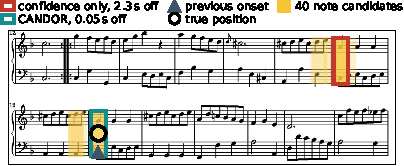
\includegraphics[width=\columnwidth]{figs/fig_example.pdf}
  \caption{One instant of a real room-microphone recording. In yellow, 40 of the
  candidate positions the detector scores. The most confident (red) lies on the
  wrong staff, 2.3\,s from the truth; \sys{} (teal) takes a less confident
  candidate on the true note (ring). The correct position was available and was
  not chosen, which is the characteristic failure on real audio.}
  \label{fig:example}
\end{figure}

\section{Method}
\label{sec:method}

\subsection{Backbone}
\label{ssec:backbone}

Every sheet-image follower of the last five years shares one perception module,
a convolutional network over the score page whose feature maps are modulated by
the audio. The mechanism is feature-wise linear
modulation~\cite{perez2018film}, which injects an external vector into a
network by scaling and shifting its activations,
\begin{equation}
  f_{\mathrm{FiLM}}(x)=s(z)\odot x+t(z),
  \label{eq:film}
\end{equation}
where $s$ and $t$ are learned linear maps of a conditioning vector $z$ and
$\odot$ is elementwise. The page alone cannot say where the performer is, so
$z$ carries the recent audio and the visual features become a function of what
has just been heard.

CYOLO~\cite{henkel2021eusipco} encodes the last two seconds of audio into $z$
with a spectrogram network and places FiLM layers through the downscale and
upscale blocks of a YOLO detector, which then predicts a bounding box for the
notehead currently sounding. CYOLO-SB~\cite{henkel2021frontiers} keeps that
arrangement and adds heads for the enclosing system and bar, so one 
$52\times52$ feature map yields all three. CODA~\cite{yang2026coda} conditions
its own backbone the same way, at the deeper stages, before cascading selection
over layout regions supplied with the score.

We take this module as given rather than as a design choice, and use the
released CYOLO detectors to propose noteheads. No detector weight is updated
anywhere in this work, and three separately trained instances are used, so the
conclusions concern the family and not one checkpoint.

\subsection{\sys{}}
\label{ssec:candor}

\sys{} sits after the backbone and replaces only its final step. Where the
detector reports the single most confident box, \sys{} treats the boxes as a
candidate set and decides among them, carrying its own state from one instant
to the next.

\subsubsection{Candidate positions}

A performance is processed in instants $t=1,\dots,T$. At each instant the
backbone reads the audio so far and the current page and scores note boxes
$b_i=(x_i,y_i,w_i,h_i)$ with confidence $o_i$; we keep the $K=256$ most
confident, $\mathcal{C}_t$. Staves are concatenated along one horizontal axis,
the unrolled coordinate $u_i$, so positions across a line break are adjacent.
The released detectors score 8,112 boxes per instant and report
\begin{equation}
  \hat{\imath}_t=\arg\max_{i\in\mathcal{C}_t} o_i ,
  \label{eq:argmax}
\end{equation}
which is the degenerate selector. \sys{} reads $\mathcal{C}_t$ and its own
previous choice $\hat u_{t-1}$, and nothing else.

\subsubsection{Transition model}

Selections must form a plausible trajectory. Between instants $\Delta_t$ frames
apart the performer advances by a roughly predictable amount, so the
displacement $d_i=u_i-\hat u_{t-1}$ is scored by a floored Gaussian whose mean
grows with elapsed time,
\begin{equation}
  \log\pi_i=\max\Big(-\frac{(d_i-\mu\rho_t)^2}{2\sigma^2},\,J\Big),
  \label{eq:prior}
\end{equation}
with $\rho_t=\mathrm{clip}(\Delta_t/\Delta_0,\,0.2,\,8)$ and $\Delta_0=5$
frames, the mean inter-onset gap in training. The floor $J$ keeps a jump
possible at bounded cost. Combined with confidence, $h_i=\log o_i+\log\pi_i$
already recovers a large part of the gap on its own.

\subsubsection{Set-based scorer}

The transition model treats candidates independently given the history. What it
cannot express is comparative, whether this box, among those on offer in this
instant, looks like a real notehead rather than a spurious response. Each
candidate is described by $\phi_i\in\mathbb{R}^{33}$ holding its confidence
relative to the instant's best, box geometry, motion relative to the history,
relation to any coarse regions the backbone emits, and a neighbourhood group
describing how crowded and how typical the box is among its neighbours. We also
read $f_i$, the 128-dimensional FiLM-conditioned feature from which the
detection head scored the box, so the decision sees the representation
perception used. A permutation-invariant network~\cite{zaheer2017deepsets}, as
in learned re-scoring of detections~\cite{hosang2017nms}, embeds the set and
pools a context shared by all candidates,
\begin{align}
  e_i &= g\big([\phi_i;\,\mathrm{ReLU}(Wf_i)]\big),\quad
  c=\Big[\tfrac{1}{K}{\textstyle\sum_j} e_j;\ \max_j e_j\Big],
  \label{eq:embed}\\
  s_i &= r\big([e_i;\,c]\big),
  \label{eq:score}
\end{align}
with $g$ and $r$ two-layer perceptrons (64, 32 and 64, 1) and
$W\in\mathbb{R}^{64\times128}$. The maximum is taken per dimension, so every
candidate is judged against its competitors.

\subsubsection{Training and inference}

The decision is supervised listwise. With $\varepsilon_i$ the error in frames of
candidate $i$, the target is $q_i\propto\exp(-\varepsilon_i/\tau)$, $\tau=3$,
and
\begin{equation}
  \mathcal{L}=-\sum_{i\in\mathcal{C}_t} q_i\,\log\frac{\exp s_i}{\sum_{j}\exp s_j},
  \label{eq:loss}
\end{equation}
so the scorer learns to order a set rather than to regress a coordinate.
History features come from previous decisions, perturbed on 30\% of samples by
Laplace noise of scale 30\,px to expose training to the drift of sequence
prediction~\cite{bengio2015scheduled}. At inference \sys{} decides
\begin{equation}
  \hat{\imath}_t=\arg\max_{i\in\mathcal{C}_t}\ \beta\,s_i+(1-\beta)\,h_i ,
  \label{eq:decode}
\end{equation}
causally and greedily, one pass over 256 candidates per instant, in 1.25\,ms on
a single CPU thread against the 50\,ms available at 20\,fps. Training on the
residual $s_i-h_i$ and deciding $\arg\max_i(s_i+h_i)$ is Eq.~\ref{eq:decode} at
$\beta=0.5$ and eliminates all four constants.

\section{Experimental setup}
\label{sec:setup}

\subsection{Dataset}

The decision model is trained on 353 pieces of
MSMD~\cite{dorfer2018msmd}, synthesized and convolved with measured room
impulse responses~\cite{traer2016}, and validated on 19, using AdamW
($3\cdot10^{-3}$, cosine, 40 epochs, batch 256). The evaluation set is the
real-performance benchmark of~\cite{henkel2019rl}: 16 pieces, 25 pages and
4,149 onsets on a Yamaha AvantGrand N2 captured with a room microphone. A
held-out set of 80 further pieces is rendered with a real impulse response and
noise from 12 to 0.5\,dB SNR.

We report the ratio of onsets whose predicted position maps to within
0.05 to 5\,s of the true time, 0.5\,s primary, with 95\% intervals bootstrapped
over pieces~\cite{efron1993}.

The four constants $(\mu,\sigma,J,\beta)$ are fitted leave-one-piece-out. For
each evaluation piece they are chosen on the other 15, pieces weighted equally,
so none influences its own decoding, and the residual variant needs no fit at
all. Seeds move results by about a point, so rows are seed means with
deviations.

\begin{table*}[t]
\centering
\caption{Real piano recordings, 16 pieces and 4,149 onsets, Yamaha AvantGrand N2
captured with a room microphone. Ratio of onsets tracked within each error
threshold. $^\dagger$\,perception model trained with additional proprietary
recordings, public checkpoint. Layout means system and bar annotations
required at test time. $\Delta$ is the gain at 0.5\,s over the perception model
the row is built on. Published figures as reported in~\cite{yang2026coda}.}
\label{tab:main}
\setlength{\tabcolsep}{4.2pt}
{\small
\begin{tabular}{lccccccc}
\toprule
& \multicolumn{5}{c}{Onset error threshold (s)} & & \\
\cmidrule(lr){2-6}
Method & $\le$0.05 & $\le$0.1 & $\le$0.5 & $\le$1.0 & $\le$5.0 & Layout & $\Delta$ \\
\midrule
MM-Loc~\cite{dorfer2016}                         & .364 & .406 & .585 & .611 & .735 & no  & \\
RL agent~\cite{henkel2019rl}                     & .185 & .200 & .476 & .603 & .901 & no  & \\
CUNet~\cite{henkel2020cunet}                     & .113 & .125 & .224 & .266 & .443 & no  & \\
CYOLO~\cite{henkel2021eusipco}                   & .563 & .581 & .712 & .749 & .919 & no  & \\
CYOLO-SB~\cite{henkel2021frontiers}              & .610 & .630 & .799 & .832 & .960 & no  & \\
CYOLO-SB+A$^\dagger$~\cite{henkel2021frontiers}  & .682 & .706 & .865 & .891 & .981 & no  & \\
CODA~\cite{yang2026coda}                         & .721 & .743 & .883 & .914 & .987 & yes & \\
\midrule
\sys{} on CYOLO                                  & .726 & .747 & .916 & .950 & .991 & no & $+$20.4 \\
\sys{} on CYOLO-SB                               & .690 & .714 & .906 & .942 & .982 & no & $+$10.7 \\
\sys{} on CYOLO-SB+A$^\dagger$                   & \textbf{.760} & \textbf{.785} & \textbf{.944} & \textbf{.969} & \textbf{.996} & no & $+$7.9 \\
\bottomrule
\end{tabular}}
\end{table*}

\section{Results}
\label{sec:results}

\begin{figure}[t]
  \centering
  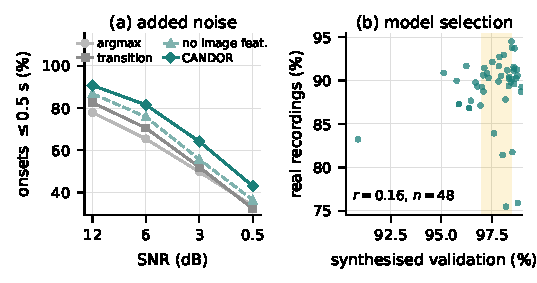
\includegraphics[width=\columnwidth]{figs/fig_analysis.pdf}
  \caption{(a) Every step from the deployed rule to the ceiling on the real
  recordings; \sys{} to the row given the true history is drift, above it is
  ranking. (b) Each point is one of 48 trained models, accuracy on synthesised
  validation audio against accuracy on the real recordings.}
  \label{fig:analysis}
\end{figure}

Table~\ref{tab:main} sets \sys{} against the published literature on the same
recordings. It tracks 94.4\% of onsets within 0.5\,s, where the previous best was 88.3\%,
and leads at every threshold. The margin is not an artifact of one perception
model. Retrained on whichever candidates each model emits, the decision gains
20.4, 10.7 and 7.9 points on three of them, and on the weakest, whose training
data is entirely public, it passes the point at which the strongest one begins.
A decision model does not need good proposals, only proposals containing the
answer. On the 94 synthetic test pieces \sys{} reaches .955 where argmax
reaches .893, and on 80 held-out pieces under a real impulse response and noise
it beats the transition model at every level from 12 to 0.5\,dB.

The tightest thresholds qualify this. On CYOLO-SB candidates \sys{} reaches
.690 and .714 at 0.05 and 0.1\,s, below CODA's .721 and .743, because a
decision is only as precise as the boxes it chooses between. Deciding recovers
which notehead, not where within it.

Table~\ref{tab:transfer} separates the parts: the transition model alone, with
no learned parameters, accounts for roughly half the gain, and the residual
variant, which fits no constant to any evaluation data, still reaches 88.7\%.

\begin{table}[t]
\centering
\caption{Components of \sys{}, cross-validated per piece on the real recordings
at 0.5\,s. argmax is Eq.~\ref{eq:argmax} over the same candidates,
$+$transition adds Eq.~\ref{eq:prior}, full adds the scorer.}
\label{tab:transfer}
\setlength{\tabcolsep}{4pt}
{\footnotesize
\begin{tabular}{lrrrr}
\toprule
 & $n$ & argmax & $+$transition & full \\
\midrule
\multicolumn{5}{l}{\emph{Perception model}}\\
CYOLO~\cite{henkel2021eusipco}          & 3 & 71.3 & 72.5 & 91.6\,$\pm$\,1.4 \\
CYOLO-SB~\cite{henkel2021frontiers}     & 6 & 80.0 & 86.5 & 90.6\,$\pm$\,0.9 \\
CYOLO-SB+A$^\dagger$                    & 3 & 86.5 & 90.8 & \textbf{94.4\,$\pm$\,0.9} \\
\midrule
\multicolumn{5}{l}{\emph{Decision model, on CYOLO-SB candidates}}\\
residual, no fitted constants           & 3 & 80.0 & 86.5 & 88.7\,$\pm$\,0.9 \\
without temporal history                & 3 & 80.0 & 86.5 & 83.7\,$\pm$\,0.4 \\
\midrule
\multicolumn{5}{l}{\emph{Image features $f_i$ read by the scorer}}\\
FiLM-conditioned backbone               & 6 & 80.0 & 86.5 & 90.6\,$\pm$\,0.9 \\
DINOv2~\cite{oquab2024dinov2}           & 1 & 80.0 & 86.5 & 90.9 \\
none                                    & 1 & 80.0 & 86.5 & 90.9 \\
\bottomrule
\end{tabular}}
\end{table}

\begin{table}[t]
\centering
\caption{Recovery from 41 discontinuities spliced into the real recordings,
on CYOLO-SB+A candidates. rec@1 is the fraction first tracked correctly within
1\,s, post the onsets tracked within 1\,s over the following 5\,s.}
\label{tab:jump}
\setlength{\tabcolsep}{4pt}
{\footnotesize
\begin{tabular}{lcccc}
\toprule
& \multicolumn{2}{c}{break present} & \multicolumn{2}{c}{no break} \\
\cmidrule(lr){2-3}\cmidrule(lr){4-5}
Decision rule & rec@1 & post & rec@1 & post \\
\midrule
argmax \eqref{eq:argmax}          & 0.27 & \textbf{0.27} & 0.15 & \textbf{0.26} \\
\sys{}                            & 0.00 & 0.08 & 0.00 & 0.09 \\
\quad $+$ silence trigger         & 0.15 & 0.17 & 0.00 & 0.09 \\
\quad $+$ confidence trigger      & 0.10 & 0.26 & 0.02 & 0.23 \\
\bottomrule
\end{tabular}}
\end{table}

\subsection{What the decision depends on}
\label{ssec:abl}

Giving the scorer the FiLM-conditioned backbone
feature, DINOv2 patch features~\cite{oquab2024dinov2} on the same grid, or no
image feature at all yields 90.6, 90.9 and 90.9, a spread well inside the
0.9-point seed deviation. On synthesized validation audio the same three differ
by 3.4 points, so those features are learnable and useful there and worth
nothing on real audio. We rebuilt the perception model with a different
audio encoder twice: a frozen MERT-95M tower~\cite{li2024mert} with only a
projection trained, which reaches 46.2 against 90.6 and overfits 12.6-fold on
the 353 training pieces, and the two-layer causal Mamba of~\cite{yang2026coda}
trained from scratch as they train it, which reaches \tbd{.}. The two are not matched on pretraining and fail
differently, on generalisation and on capacity, arriving at the same place.
Replacing the visual stem with frozen DINOv2-base patches on the same
$52\times52$ grid, against a control retrained identically, gives \tbd{.}.

Removing the features computed against the previous
decision costs 7.2 points, the largest single ablation here. Teacher forcing
attributes two thirds of the remaining error to drift, since given the true previous
position the same scorer reaches 98.0\% against the causal oracle's 99.6\%
(Fig.~\ref{fig:analysis}a). The sequence is hard, not the image.

Across 48 trained
models, accuracy on the synthesized validation split correlates $r=0.16$ with
accuracy on the real recordings (Fig.~\ref{fig:analysis}b); the
best-validation model scores 89.3 on real audio, below one reading no image
features at all. A reverberant held-out set does better ($r=0.80$) and still
mispicks. Since the whole field selects models on synthesized audio, this is a
caution beyond our own experiments, and it is why our constants are
cross-validated on the target recordings instead.


\subsection{Where the forward assumption fails}
\label{ssec:jump}

Eq.~\ref{eq:prior} assumes the performance moves forward, which is why the
decision is tractable and also why a repeat or a jump breaks it. Following the
protocol of~\cite{yang2026coda} we splice three discontinuities into each
performance at random destinations, re-running perception on the spliced audio
so its conditioning is genuinely wrong afterwards, and excluding jumps across a
page boundary where state resets anyway, leaving 41.

Table~\ref{tab:jump} reports a systematic failure. After a jump \sys{} is far
worse than the rule it replaces, 0.08 against 0.27 of onsets tracked over the
next five seconds, because the transition model holds the trajectory at a stale
position. Suppressing it on detected silence helps where a break exists and not
otherwise, as its design implies; triggering on the scorer's own confidence
needs no break and recovers most of the loss, but never beats argmax; the same
ordering holds over 220 jumps on the synthetic benchmark. A transition
model strong enough to be worth ten points on continuous playing is strong
enough to be wrong at a discontinuity, and reconciling the two is open.

\section{Conclusion}
\label{sec:conclusion}

The synthetic-to-real gap in sheet-image score following has been read as a
perception failure. It is a decision failure: a correct position is already
among the candidates at every onset, and choosing among them in real time takes real
piano recordings from 80.0\% to 94.4\%, against 88.3\% previously.

\vfill\pagebreak

\noindent Limitations. The correct page is given, all performances are
piano, and 16 evaluation pieces cannot resolve differences of a point.

\section{Compliance with ethical standards}
\label{sec:ethics}
This is a numerical study that uses only publicly available data; no ethical
approval was required.

\section{Acknowledgments}
\label{sec:ack}
This research was enabled in part by support provided by Calcul Qu\'ebec and
the Digital Research Alliance of Canada. \tbd{Funding sources.}

{\footnotesize
\bibliographystyle{IEEEbib}
\bibliography{refs}}

\end{document}
